

% !TEX root = NotesDeCours.tex

% ================================================================================================ 
% Page de titre :
% ================================================================================================


\part{Equations bilan}

%%%%%%%%%%%%%%%%%%%%%%%%%%%%%%%%%%%%%%%%%%%%%%%%%%%%%%%%%%%%%%%%%%%%%%%%%%%%%%%%%%%%%%%%%%
%\section{\bfseries Equations de bilan}
%%%%%%%%%%%%%%%%%%%%%%%%%%%%%%%%%%%%%%%%%%%%%%%%%%%%%%%%%%%%%%%%%%%%%%%%%%%%%%%%%%%%%%%%%%


\section*{5. Equations-bilan et régimes d'écoulement}

\begin{frame}

  \color{bleu}

  \begin{flushleft}
    
    \Large
   	\bf
    
    Mécanique des fluides 

  \end{flushleft}
  
  \ligne{3} % remplace: \noindent \thickline{0.5mm}{150}

  \begin{flushright}

    \rm

    \textrm{David} \textsc{Fabre}
    
    \vspace{3mm}
    
    IMFT / UPS
    
    Département de Mécanique
    


  \end{flushright}

\begin{picture}(110, 25)(12, -20)
  \put( 15, -22){\includegraphics[width=65mm]{./Figures/MBG_fig19.png}}
  \put(84, -12){\color{gris} \slshape \small Interaction entre deux}    	
  \put(84, -15){\color{gris} \slshape \small tourbillons contrarotatifs}
  \put(84, -19){\color{gris} \slshape \small \rm \copyright\ \! P. Brancher, IMFT}
  \put(16, 3){\color{gris} $(a)$}
  \put(16, -14){\color{gris} $(b)$}
  \put(74, 7){\color{gris} $(c)$}
  \put(74, -12){\color{gris} $(d\, )$}
\end{picture}
  \vspace{7mm}
  
  \begin{flushright}
    
    \Large
   	\bf
    
    5. Equations-bilan et régimes d'écoulements

  \end{flushright}

\end{frame}

%%%%%%%%%%%%%%%%%%%%%%%%%%%%%%%%%%%%%%%%%%%%%%%%%%%%%%%%%%%%%%%%%%%%%%%%%%%%%%%%%%%%%%%%%%
% Sommaire :
%%%%%%%%%%%%%%%%%%%%%%%%%%%%%%%%%%%%%%%%%%%%%%%%%%%%%%%%%%%%%%%%%%%%%%%%%%%%%%%%%%%%%%%%%%


\begin{frame}{Sommaire}

\small
  
\hspace*{2mm}
\begin{tabular}{cc}
		%&
  		\begin{minipage}{62mm}
  			\tableofcontents[firstsection=-2]
      \vspace{15mm}
  		\end{minipage}
  		&   
  		\begin{minipage}{60cm}
		  \vspace*{-5mm}  
  			%\includegraphics[width=40mm]{vagues.jpg} 
  		\end{minipage}
  	\end{tabular}

\vspace{0mm}

\end{frame}


\subsection{ Equations-bilan  sous forme locale et intégrale}

\subsubsection{Equations-bilan : généralités}

%-----------------------------------------------------------------------------------------
\begin{frame}{Les différents types de systèmes}
%-----------------------------------------------------------------------------------------

\small

\begin{itemize}%[<+-| alert@+>]
\item<1->
On appelle \textcolor{vert}{\bf système isolé} tout système qui n'échange pas avec l'extérieur
($\mydot{F}_e=0$) : \\ ni matière, ni quantité de mouvement, ni travail, ni chaleur.
\item<2->
On appelle \textcolor{rouge}{\bf matériel} ${\cal D}(t)$ un volume constitué des mêmes particules fluides, 
suivi au cours du temps.
C'est donc un concept Lagrangien et l'équivalent d'un système \textcolor{rouge}{\bf fermé},
qui n'échange pas de matière avec l'extérieur mais qui peut cependant échanger 
de la quantité de mouvement, du travail ou de la chaleur.
\item<11->
On appelle \textcolor{bleu}{\bf volume de contrôle} $\Omega$ un volume fixe dont
la frontière peut être traversée par de la matière entrante et sortante.
Il s'agit donc d'un concept Eulerien équivalent à un système \textcolor{bleu}{\bf ouvert} 
qui peut échanger matière, quantité de mouvement, travail et chaleur avec l'extérieur.


\end{itemize}

\medskip

\begin{overprint}

\onslide<3>

\begin{center}
\begin{picture}(60, 35)(0, -5)
\put(0, 0){\includegraphics[width=60mm]{volume_materiel1.png}}
\put(22, -5){\color{rouge} Volume matériel $\mathcal{D}(t)$}
\end{picture}
\end{center}

\onslide<4>

\begin{center}
\begin{picture}(60, 35)(0, -5)
\put(0, 0){\includegraphics[width=60mm]{volume_materiel2.png}}
\put(22, -5){\color{rouge} Volume matériel $\mathcal{D}(t)$}
\end{picture}
\end{center}

\onslide<5>

\begin{center}
\begin{picture}(60, 35)(0, -5)
\put(0, 0){\includegraphics[width=60mm]{volume_materiel3.png}}
\put(22, -5){\color{rouge} Volume matériel $\mathcal{D}(t)$}
\end{picture}
\end{center}

\onslide<6>

\begin{center}
\begin{picture}(60, 35)(0, -5)
\put(0, 0){\includegraphics[width=60mm]{volume_materiel4.png}}
\put(22, -5){\color{rouge} Volume matériel $\mathcal{D}(t)$}
\end{picture}
\end{center}

\onslide<7>

\begin{center}
\begin{picture}(60, 35)(0, -5)
\put(0, 0){\includegraphics[width=60mm]{volume_materiel5.png}}
\put(22, -5){\color{rouge} Volume matériel $\mathcal{D}(t)$}
\end{picture}
\end{center}

\onslide<8>

\begin{center}
\begin{picture}(60, 35)(0, -5)
\put(0, 0){\includegraphics[width=60mm]{volume_materiel6.png}}
\put(22, -5){\color{rouge} Volume matériel $\mathcal{D}(t)$}
\end{picture}
\end{center}

\onslide<9>

\begin{center}
\begin{picture}(60, 35)(0, -5)
\put(0, 0){\includegraphics[width=60mm]{volume_materiel7.png}}
\put(22, -5){\color{rouge} Volume matériel $\mathcal{D}(t)$}
\end{picture}
\end{center}

\onslide<10>

\begin{center}
\begin{picture}(60, 35)(0, -5)
\put(0, 0){\includegraphics[width=60mm]{streamlines_car.jpg}}
\end{picture}
\end{center}

\onslide<11>

\begin{center}
\begin{picture}(60, 35)(0, -5)
\put(0, 0){\includegraphics[width=60mm]{streamlines_car1.jpg}}
\put(8, 0.5){\color{bleu} \linethickness{0.5mm} \framebox(46, 24){}}
\put(22, -5){\color{bleu} Volume de contrôle $\Omega$}
\end{picture}
\end{center}

\onslide<12>

\begin{center}
\begin{picture}(60, 35)(0, -5)
\put(0, 0){\includegraphics[width=60mm]{streamlines_car2.jpg}}
\put(8, 0.5){\color{bleu} \linethickness{0.5mm} \framebox(46, 24){}}
\put(22, -5){\color{bleu} Volume de contrôle $\Omega$}
\end{picture}
\end{center}

\onslide<13>

\begin{center}
\begin{picture}(60, 35)(0, -5)
\put(0, 0){\includegraphics[width=60mm]{streamlines_car3.jpg}}
\put(8, 0.5){\color{bleu} \linethickness{0.5mm} \framebox(46, 24){}}
\put(22, -5){\color{bleu} Volume de contrôle $\Omega$}
\end{picture}
\end{center}

\onslide<14>

\begin{center}
\begin{picture}(60, 35)(0, -5)
\put(0, 0){\includegraphics[width=60mm]{streamlines_car4.jpg}}
\put(8, 0.5){\color{bleu} \linethickness{0.5mm} \framebox(46, 24){}}
\put(22, -5){\color{bleu} Volume de contrôle $\Omega$}
\end{picture}
\end{center}

\onslide<15>

\begin{center}
\begin{picture}(60, 35)(0, -5)
\put(0, 0){\includegraphics[width=60mm]{streamlines_car5.jpg}}
\put(8, 0.5){\color{bleu} \linethickness{0.5mm} \framebox(46, 24){}}
\put(22, -5){\color{bleu} Volume de contrôle $\Omega$}
\end{picture}
\end{center}

\onslide<16>

\begin{center}
\begin{picture}(60, 35)(0, -5)
\put(0, 0){\includegraphics[width=60mm]{streamlines_car6.jpg}}
\put(8, 0.5){\color{bleu} \linethickness{0.5mm} \framebox(46, 24){}}
\put(22, -5){\color{bleu} Volume de contrôle $\Omega$}
\end{picture}
\end{center}

\onslide<17>

\begin{center}
\begin{picture}(60, 35)(0, -5)
\put(0, 0){\includegraphics[width=60mm]{streamlines_car7.jpg}}
\put(8, 0.5){\color{bleu} \linethickness{0.5mm} \framebox(46, 24){}}
\put(22, -5){\color{bleu} Volume de contrôle $\Omega$}
\end{picture}
\end{center}

\onslide<18>

\begin{center}
\begin{picture}(60, 35)(0, -5)
\put(0, 0){\includegraphics[width=60mm]{streamlines_car8.jpg}}
\put(8, 0.5){\color{bleu} \linethickness{0.5mm} \framebox(46, 24){}}
\put(22, -5){\color{bleu} Volume de contrôle $\Omega$}
\end{picture}
\end{center}

\onslide<19>

\begin{center}
\begin{picture}(60, 35)(0, -5)
\put(0, 0){\includegraphics[width=60mm]{streamlines_car9.jpg}}
\put(8, 0.5){\color{bleu} \linethickness{0.5mm} \framebox(46, 24){}}
\put(22, -5){\color{bleu} Volume de contrôle $\Omega$}
\end{picture}
\end{center}

\onslide<20>

\begin{center}
\begin{picture}(60, 35)(0, -5)
\put(0, 0){\includegraphics[width=60mm]{streamlines_car10.jpg}}
\put(8, 0.5){\color{bleu} \linethickness{0.5mm} \framebox(46, 24){}}
\put(22, -5){\color{bleu} Volume de contrôle $\Omega$}
\end{picture}
\end{center}

\onslide<21>

\begin{center}
\begin{picture}(60, 35)(0, -5)
\put(0, 0){\includegraphics[width=60mm]{streamlines_car11.jpg}}
\put(8, 0.5){\color{bleu} \linethickness{0.5mm} \framebox(46, 24){}}
\put(22, -5){\color{bleu} Volume de contrôle $\Omega$}
\end{picture}
\end{center}

\end{overprint}

\vspace{5mm}

\end{frame}


%--------------------------------------------------------------------------------------------------
\begin{frame}{Théorème du transport (Rappel chap. 3)}

%--------------------------------------------------------------------------------------------------

\small

Les équations de la physique (bilans de masse, de quantité de mouvement, d'énergie), s'écrivent naturellement en considérant un volume matériel  ${\cal D} (t)$.

\smallskip

Le théorème de Transport permet de traduire ce bilan dans le cas (Eulérien) d'un volume de contrôle $\Omega$.



\smallskip

{\bf Théorème :} 


Considérons un {\em domaine matériel } mobile ${\cal D} (t)$ coïncidant à l'instant $t$ avec un {\em volume de contrôle } fixe $\Omega$ (bordé par un countour $\partial \Omega$).

$$
\includegraphics[width=.45\linewidth]{Theoreme_de_transport.png}
$$



La dérivée matérielle de la quantité intégrale $F(t) =  \int_{{\cal D}(t)} f d V$ s'écrit alors  :

$$
\frac{d}{dt} \int_{{\cal D}(t)} f d V  = \int_\Omega \frac{\partial f } {\partial t} dV + \oint_{\partial\Omega} f\myvec{u}\cdot\myvec{n}\, dS
$$


\medskip
\pause




%$\longrightarrow$ $ \displaystyle \int_\Omega \dpdt{f}\, dV$ correspond à la variation temporelle de la quantité $f$
%dans le volume $\Omega$.

%\smallskip

%$\longrightarrow$ $\displaystyle \oint_{\partial\Omega} f\myvec{u}\cdot\myvec{n}\, dS$ correspond au \textcolor{rouge}{flux}
%de la quantité $f$ à travers la frontière de $\Omega$.

%\pause
%\bigskip


{\em Remarque :} ce théorème est une généralisation du théorème suivant pour un problème monodimensionnel :

$$
\frac{d}{dt} \int_{a(t)}^{b(t)} f(x,t) dx = \int_{a(t)}^{b(t)}  \frac{\partial f}{\partial t} d x + \left[ \frac{d b}{dt} f(b(t),t)  - \frac{d a}{dt} f(a(t),t) \right]
$$


{\color{green} Démonstration :}

\end{frame}


 
%==========================================================================================
\subsubsection{Bilan de masse}
%==========================================================================================

%-----------------------------------------------------------------------------------------
%\subsubsection{bilans intégraux}
%-----------------------------------------------------------------------------------------
\begin{frame}{Bilan de masse : bilans intégraux}
%-----------------------------------------------------------------------------------------

\small



Quantité physique : \textbf{masse} $M$ associée à la grandeur intensive $\rho$ (\textbf{masse volumique}).

\bigskip

Pour un volume matériel $\mathcal{D}(t)$ donné 
$$
	M(t, \mathcal{D}) = \int_{\mathcal{D}(t)} \rho(\myvec{x}, t) \, dV
$$

\medskip 

\pause

Pour ce système matériel, le principe de conservation de la masse $\ddt{M} = 0$ s'écrit :

\medskip

\begin{itemize}
\item
	bilan intégral lagrangien pour le volume matériel $\mathcal{D}$ en suivant le fluide
	dans son mouvement
	\begin{equation}
		\color{rouge}
		\ddt{} \int_{\mathcal{D}(t)} \rho(\myvec{x}, t) \; dV 
		= 0
		\label{eq:bilan_global_lagrangien_masse}
	\end{equation}
\medskip

\pause

\item
  bilan intégral eulérien pour le volume de contrôle fixe $\Omega$ (système ouvert)
	\begin{equation}
		\color{rouge}
		\dpdt{} \int_{\Omega} \rho(\myvec{x}, t) \; dV 
		=
		- \oint_{\partial \Omega} \rho \,  \myvec{u}\cdot \myvec{n} \, dS
		\label{eq:bilan_global_eulerien_masse}
	\end{equation}
\end{itemize}

{\color{vert} [Démonstration] :} théorème de transport avec $f= \rho$

\pause
\medskip


\vspace{0mm}

\end{frame}

%-----------------------------------------------------------------------------------------
%\subsubsection{bilans locaux}
%-----------------------------------------------------------------------------------------
\begin{frame}{Bilan de masse : bilans locaux}
%-----------------------------------------------------------------------------------------

\small

A partir des bilans intégraux précédents, on déduit les équations locales de bilan de masse :

\medskip

\begin{itemize}

\item
  Bilan local eulérien
	\begin{equation}
			\color{rouge}
		\dpdt{\rho} + \divergence ( \rho \, \myvec{u}\ ) = 0
		\label{eq:bilan_local_eulerien_masse}
	\end{equation}
\medskip

\pause 
\textcolor{vert}{[Démonstrations :]}

\begin{itemize}
	\item $(i)$ A partir du bilan intégral Eulérien, à l'aide du théorème de la divergence
	\item $(ii)$ Directement par un bilan sur un volume élémentaire 
\end{itemize}


\pause

\item
	Bilan local lagrangien, en suivant la particule fluide dans son mouvement
	\begin{equation}
		\color{rouge}
		\ddt{\rho} + \rho \, \divergence \myvec{u} = 0
		\label{eq:bilan_local_lagrangien_masse}
	\end{equation}
\pause

\textcolor{vert}{[Démonstrations :] }
\begin{itemize}
	\item $(i)$ En utilisant la définition de la dérivée particulaire
	\item $(ii)$ En variables lagrangiennes (cf. MMC) 
\end{itemize}


\end{itemize}
\end{frame}


%==========================================================================================
\subsubsection{Bilan de quantité de mouvement}
%==========================================================================================

%-----------------------------------------------------------------------------------------
%\subsubsection{Bilans intégraux}
%-----------------------------------------------------------------------------------------
\begin{frame}{Bilan de quantité de mouvement : bilans intégraux}
%-----------------------------------------------------------------------------------------

\small

Quantité physique : quantité de mouvement $\myvec{Q}$ associée à la grandeur intensive 
$\rho \, \myvec{u}$.

\medskip

Pour un volume matériel $\mathcal{D}(t)$ donné : 
$ \displaystyle
	\myvec{Q}(t, \mathcal{D}) 
	= \int_{\mathcal{D}(t)} \rho(\myvec{x}, t)\, \myvec{u}(\myvec{x}, t) \, dV
$

\pause

Principe de conservation de la quantité de mouvement : 
$\ddt{\myvec{Q}} = \myvec{F}\indice{ext $\rightarrow \mathcal{D}$}$

\smallskip

\begin{itemize}
\item
	bilan intégral lagrangien pour le volume matériel $\mathcal{D}$ en suivant le fluide
	dans son mouvement
	\begin{equation}
		\color{rouge}
		\ddt{} \int_{\mathcal{D}(t)} \rho \, \myvec{u} \; dV 
		=
		\int_{\mathcal{D}(t)} \rho \myvec{g} \, dV 
		+ \oint_{\partial \mathcal{D}(t)} 
		\left( -p \myvec{n} + \mytensor{\tau} \cdot \myvec{n}\right) \; dS
		\label{eq:bilan_global_lagrangien_qdm}
	\end{equation}
	où $\myvec{g}$ désigne la gravité (ou toute force à distance par unité de masse).
	
	et où les forces surfaciques sont la pression (normale) et la contrainte visqueuse (représentée par le tenseur $\mytensor{\tau}$).
	Ce bilan s'interprète simplement comme le \textcolor{vert}{principe fondamental de la dynamique} 
	appliqué au système matériel $\mathcal{D}$.

\smallskip

\pause
\item
  bilan intégral eulérien pour le volume de contrôle fixe $\Omega$ (système ouvert)
	\begin{equation}
		\color{rouge}
		\dpdt{} \int_{\Omega} \rho \, \myvec{u} \; dV 
		=
		\int_{\Omega} \rho \myvec{g} \, dV 
		+ \oint_{\partial \Omega} \left( -p \myvec{n} + \mytensor{\tau} \cdot \myvec{n}\right) \; dS
		- \oint_{\partial \Omega} \rho \, \myvec{u}\; (\myvec{u}\cdot \myvec{n}) \, dS
		\label{eq:bilan_global_eulerien_qdm}
	\end{equation}
\end{itemize}

{\color{vert} [Démonstration] :} théorème de transport avec $f= \rho \myvec{u}$

\medskip
\pause

\color{gris} Remarque : en présence d'interface traversant la frontière du volume considéré, il faut ajouter au membre de droite la contribution de la force de tension superficielle
$$
\int_{\mathcal{L}} \gamma \myvec{n}_{\cal L} \, dl
$$

%\vspace{0mm}

\end{frame}
%-----------------------------------------------------------------------------------------
%\subsubsection{Bilans locaux}
%%-----------------------------------------------------------------------------------------
%\begin{frame}{Bilan de quantité de mouvement : bilans locaux}
%%-----------------------------------------------------------------------------------------
%
%\small
%
%En utilisant le théorème de la divergence sur le bilan intégral lagrangien, et en écrivant ce bilan
%pour un volume matériel infinitésimal $dV$, de masse $dm = \rho dV$, 
%on déduit les équations locales de bilan de quantité de mouvement :
%
%\medskip
%\pause
%
%\begin{itemize}
%\item
%	Bilan local lagrangien, en suivant la particule fluide dans son mouvement :
%	\begin{equation}
%		\mbox{\textcolor{gris}{[Démonstration] \quad $\longrightarrow$ \quad}}
%		\rho \ddt{\myvec{u}} 
%		= 
%		\rho \myvec{f} + \divergence \mytensor{\sigma}
%		%\label{eq:bilan_local_lagrangien_qdm}
%	\end{equation}
%	
%	\medskip
%	En multipliant par le volume de la particule fluide, ce bilan local s'interprète comme
%	\\ le \textcolor{vert}{principe fondamental de la dynamique} appliqué à la particule fluide.
%
%	\pause
%
%	\bigskip
%	En écrivant que pour un fluide $\mytensor{\sigma} = -p \mytensor{1} + \mytensor{\tau}$,
%	le bilan local donne l'équation de Navier-Stokes généralisée :
%	\begin{equation}
%		\color{rouge}
%		\rho \ddt{\myvec{u}} 
%		= 
%		\rho \myvec{f} - \gradient p + \divergence \mytensor{\tau}
%		\label{eq:bilan_local_lagrangien_qdm}
%	\end{equation}
%
%\bigskip
%\pause
%
%\item
%  Bilan local eulérien : on déduit directement de l'expression précédente
%	\begin{equation}
%		\rho \left [ \dpdt{\myvec{u}} + \left ( \myvec{u} \cdot \gradient\ \right ) \myvec{u} \right ]
%		= \rho \myvec{f} + \divergence \mytensor{\sigma}
%		%\label{eq:bilan_local_eulerien_qdm}
%	\end{equation}
%	ou encore
%	\begin{equation}
%		\color{rouge}
%		\rho \left [ \dpdt{\myvec{u}} + \left ( \myvec{u} \cdot \gradient\ \right ) \myvec{u} \right ]
%		= \rho \myvec{f} - \gradient p + \divergence \mytensor{\tau}
%		\label{eq:bilan_local_eulerien_qdm}
%	\end{equation}
%\end{itemize}
%
%
%\vspace{15mm}
%
%\end{frame}

%-----------------------------------------------------------------------------------------
%\subsubsection{Bilans locaux}
%-----------------------------------------------------------------------------------------
\begin{frame}{Bilan de quantité de mouvement : bilans locaux}
%-----------------------------------------------------------------------------------------

\small

%En utilisant le théorème de la divergence sur le bilan intégral lagrangien, et en écrivant ce bilan
%pour un volume matériel infinitésimal $dV$, de masse $dm = \rho dV$, 
%on déduit les équations locales de bilan de quantité de mouvement :

\medskip
\pause

\begin{itemize}
\item
  Bilan local eulérien ou "sous forme conservative"

	\begin{equation}
		\color{rouge}
		\left[ \dpdt{} (\rho \myvec{u}) +  \myvec{\divergence}(\rho \myvec{u} \otimes \myvec{u}) \right] 
		= \rho \myvec{g} - \gradient p + \myvec{\divergence}( \mytensor{\tau} )
		\label{eq:bilan_local_eulerien_qdm}
	\end{equation}

\pause 
\medskip

{\color{vert} [Démonstration] :}

 A partir du bilan intégral eulérien, à l'aide du théorème de la divergence.

\pause
\medskip

\item
	Bilan local lagrangien, 
	\begin{equation}
	\color{rouge}
		\rho \ddt{\myvec{u}} 
		= 
		\rho \myvec{g}  - \gradient p + \myvec{\divergence}( \mytensor{\tau})
	\end{equation}
	
	\medskip
%	Ce bilan local s'interprète comme
%	\\ le \textcolor{vert}{principe fondamental de la dynamique} appliqué à la particule fluide.

\pause
\medskip

{\color{vert} [Démonstration] :}

$(i)$ A partir du bilan local eulérien (exercice), 

$(ii)$ Par un bilan des forces appliqué à un volume élémentaire $dV$.

\medskip
\pause

\item Autre écriture (pour un fluide Newtonien, en négligeant la viscosité en volume) :


	\begin{equation}
	\color{rouge}
		\rho \left( \dpdt{\myvec{u}} + \mytensor{grad} (\myvec{u}) \cdot \myvec{u}  \right)
		= 
		\rho \myvec{g}  - \gradient p + \mu \left( \Delta \myvec{u} + \frac{1}{3} \gradient (\divergence( \myvec{u})) \right)
	\end{equation}


Démo : exercice

\end{itemize}


\vspace{15mm}

\end{frame}

%==========================================================================================
\subsubsection{Autres équations-bilan}
%==========================================================================================




%-----------------------------------------------------------------------------------------
\begin{frame}{Autres équations-bilan :}
%-----------------------------------------------------------------------------------------
\small

Le document {\bf Formulaire de mécanique des fluides, annexe C} liste d'autres équations-bilans utiles en mécanique des fluides :

\begin{itemize}

 \item bilan intégral d'énergie totale.  
 
 {\color{gris} (Egalement appelé premier principe en système ouvert).}
 

 \item Bilan local d'énergie totale.  
 
  {\color{gris} (Se déduit du bilan intégral).}
 
 \begin{equation}
\color{rouge}
		\rho \ddt{} \left( c_v T + \frac{|\vec{u}|^2}{2} \right) 
		= \rho \vec{g} \cdot \vec{u} 
		- \gradient ( p) \cdot  \vec{u}  
		+ \divergence ( \mytensor{\tau}) \cdot \vec{u}  
		 - \divergence(\vec{q}) ; \qquad \vec{q} = - \lambda \gradient(T)
		%\label{eq:bilan_local_lagrangien_qdm}
\end{equation}


  (cf. chapitres 11-12, écoulements compressibles de gaz parfaits)
 
 
 
\item Bilan local d'énergie cinétique. 

{\color{gris} (S'obtient à partir du bilan local de QDM en projetant sur $\vec{u}$).}

(cf. chap. 7, théorème de Bernoulli).


\item bilan intégral d'énergie cinétique. 

{\color{gris} (S'obtient à partir du bilan local, en intégrant sur un volume $\Omega$).}

(cf chap. 9, perte de charge dans une conduite , et chap. 10, flux d'énergie acoustique).
 

 
 \item Bilans d'énergie interne 
 
 {\color{gris} (S'obtiennent en combinant les bilans d'énergie totale et d'énergie cinétique)}
 
 \item Bilans d'entropie (second principe en système ouvert)
 
 \item (...)
 
 \end{itemize}




%\vspace{40mm}

\end{frame}

%==========================================================================================
\subsection{Equations de Navier--Stokes}
%==========================================================================================


\begin{frame}{Equations du mouvement d'un fluide}

\small

On peut donc maintenant résumer les équations régissant le mouvement d'un fluide dans le cas le plus général :

\pause 

\begin{equation*}
\mbox{Bilan local de masse : } \quad 	\color{rouge}
		\ddt{\rho} + \rho \, \divergence \myvec{u} = 0
\end{equation*}


\begin{equation*}
\mbox{Bilan local de qdm : }   \quad 	\color{rouge}
\color{rouge}
\rho  \ddt{\myvec{u}} 
= 
\rho \myvec{g}  - \gradient p + \mu  \Delta \myvec{u} + \frac{\mu}{3} \gradient (\divergence( \myvec{u}))
\end{equation*}

 \begin{equation*}
\mbox{Bilan local d'énergie : } \quad
\color{rouge}
		\rho \ddt{} \left( c_v T + \frac{|\vec{u}|^2}{2} \right) 
		= \rho \vec{g} \cdot \vec{u} 
		- \gradient ( p) \cdot  \vec{u}  
		+ \divergence ( \mytensor{\tau}) \cdot \vec{u}  
		 +  \lambda \Delta T
		%\label{eq:bilan_local_lagrangien_qdm}
\end{equation*}

\begin{equation*}
\mbox{Equation d'état : } \quad { \color{rouge} p = \rho r T} \mbox{ (gaz parfait) ou }  \quad { \color{rouge} \rho = \rho_0} \mbox{ (liquide incompressible indilatable)} 
\end{equation*}

\end{frame}

\begin{frame}{Conditions limites}

\small

A ces équations doivent être adjointes des conditions limites sur une frontière $\Sigma$ (éventuellement mobile) séparant le fluide d'un milieu extérieur (solide ou fluide).

	\begin{center}
		\setlength{\unitlength}{0.7mm}
		\begin{picture}(90, 50)
			\put(0, 0){\includegraphics[width=63mm]{conditions_limites.png}}	
			\put(58, 39){$\myvec{n}$}
			\put(63.5, 32){milieu extérieur}
			\put(63, 27){(fluide ou solide)}
			\put(28, 17){\setlength{\fboxsep}{1mm}\colorbox{white}{$\myvec{x}$}} 
			\put(9, 24){frontière $\Sigma$}
			\put(63, 15){fluide}
		\end{picture}
	\end{center}

\end{frame}

\begin{frame}{Conditions limites}
\small

\begin{itemize}
\item Condition limite cinématique.
$$
\myvec{u}(\myvec{x} \in \Sigma, t) = \myvec{u}\indice{ext}(\myvec{x} \in \Sigma, t)
$$
Condition souvent simplifiée dans le cas ou la frontière $\Sigma$ une paroi fixe sous la forme suivante :

$$\color{red} \myvec{u} = \myvec{0}$$


\item Condition limite dynamique 

$$
\mytensor{\sigma}(\myvec{x} \in \Sigma, t) \cdot \myvec{n} 
	-
	\mytensor{\sigma}\indice{ext}(\myvec{x} \in \Sigma, t)\cdot \myvec{n}
= \gamma K \qquad \mbox{( $K = $ courbure de la surface, cf. chap. 2)}
$$


Condition souvent simplifiée dans le cas ou $\Sigma$ est une surface libre plane (d'altitude $y=cte$) sous la forme suivante :

$\mytensor{\sigma} \cdot \myvec{n}  =-  p_{ext} \myvec{n} $ 

c.a.d. { \color{rouge} $ p - \tau_{yy} = p_{ext}$}  et ${\color{rouge}  \tau_{xy} = \tau_{yz} = 0 }$

\item Condition limite thermique

$$ \myvec{q} = \myvec{q}_{ext} $$ 

Condition souvent simplifiée sous l'une des deux formes suivantes :

 { \color{rouge} $ \myvec{q} = \myvec{0} $}  ( paroi adiabatique ) ou ${\color{rouge}  T = T_{ext}}$ (paroi isotherme).

\pause
\medskip

NB : les deux premières conditions limites généralisent celles vues au chapitre 4 pour les écoulements plans parallèles.

\end{itemize}





\end{frame}


\subsection{Simplifications et régimes d'écoulement}

\subsubsection{Simplifications pour les liquides}
\begin{frame}{Simplifications (cas des liquides)}
\small

Dans le cas des liquides incompressibles, indilatables ($\rho = \rho_0)$

\begin{enumerate} 

\item L'équation-bilan de masse se simplifie en $\divergence (\myvec{u}) = 0$ .

$=>$ L'écoulement est iso-volume (on dit aussi "écoulement incompressible", par abus de language).

\item Les problèmes dynamique et thermique sont découplés (aucun terme ne dépend de $T$ dans l'équation-bilan de QDM).

$=>$ Si l'on ne s'intéresse qu'au champ de vitesse et aux forces générées sur les obstacles, on peut oublier l'équation de la température !

$=>$ en revanche si l'on s'intéresse aux transferts thermiques, il faut d'abord résoudre le problème dynamique avant de résoudre le problème thermique...
(cf. cours de transferts thermiques, chapitre "convection").

%\end{enumerate}
\end{enumerate}

\pause
\medskip

{\bf Conclusion :}  Pour les liquides incompressibles (chapitres 6 à 9) on retiendra les équations sous la forme suivante ("Equations de Navier-Stokes incompressibles") :



\begin{equation*}
\left\{
\begin{array}{l}
\color{rouge} \divergence \myvec{u} = 0
\\
\color{rouge}
\rho_0 \ddt{\myvec{u}} 
= 
\rho_0  \myvec{g}  - \gradient p + \mu  \Delta \myvec{u} 
\end{array}
\right.
\end{equation*}


%\begin{enumerate}

%\item[3] On constate que dans ces équations la pression est définie à une constante arbitraire près ($\gradient(p+Cte) = \gradient(p)$).

%=>  

\end{frame}

\begin{frame}{Simplifications (cas des liquides)}
\small

\begin{enumerate}

\item[3] Simplification sur la pression :

Les termes de gravité et de gradient de pression peuvent se regrouper en introduisant la {\em pression motrice} 
$$
\hat{p} = p - \rho_0 \vec{g} \cdot \vec{x} \quad { \color{gris} ( = p + \rho_0 g z  \mbox{ si la gravité est selon} -z) }
$$

$=>$ L'eq. de NS se réécrit alors :

$$
\rho_0 \ddt{\myvec{u}} 
= 
 - \gradient \hat{p} + \mu  \Delta \myvec{u} 
$$

Conséquences :
\begin{itemize}

\item L'écoulement d'un {\em fluide pesant} est {\em cinématiquement équivalent} à celui d'un fluide non pesant ($\vec{g}=\vec{0}$)

\item La force exercée par un fluide {\em pesant} ${\cal F}$ sur une surface $\Omega$ de frontière $\cal S$ peut être évaluée ainsi :

\begin{eqnarray*} 
\myvec{F}_{{\cal F} \longrightarrow \Omega} &=& - \oint_{\cal S} p \myvec{n} dS 
\\
&=& - \oint_{\cal S} \hat{p} \vec{n} dS + \int_{\Omega}  \gradient( \rho_0 \vec{g} \cdot \vec{x}  ) dV 
\\
&=&  - \oint_{\cal S} \hat{p} \vec{n} dS - \rho_0 \vec{g} V
\end{eqnarray*}

\item Interprétation : la force exercée sur un obstacle {\em entièrement immergé} se compose de deux termes : une {\em force hydrodynamique}
qui peut être déduite de la solution du problème {\em non pesant}, et une force hydrostatique qui n'est autre que la poussée d'Archimède !

\item Conséquence : la force horizontale sur un sous-marin {\color{gris} (ou un avion en vol subsonique comme on le verra plus tard)} ne dépend pas de $g$ ! 

(cf. chapitre 1).

 \end{itemize}
 \end{enumerate}
 
 \end{frame}


\subsubsection{Analyse dimensionnelle de l'équation-bilan de QDM}

\begin{frame}{Analyse dimensionnelle de l'eq. de QDM} 

(a finir) 

$=>$ Nombre de Reynolds

\end{frame}


\subsubsection{Analyse dimensionnelle de l'équation-bilan de masse }

\begin{frame}{Analyse dimensionnelle de l'eq. de masse} 

(a finir) 

$=>$ Nombre de Mach

\end{frame}



%
%\begin{frame}{Ecoulement incompressible de fluide newtonien}
%%-----------------------------------------------------------------------------------------
%
%\small
%
%Dans le cas général, le bilan de quantité de mouvement pour un fluide en écoulement s'écrit
%\begin{equation}
%	\color{rouge}
%	\rho \ddt{\myvec{u}} 
%	= \rho \myvec{f} + \divergence \mytensor{\sigma}
%	= \rho \myvec{f} - \gradient p + \divergence \mytensor{\tau}
%	\label{eq:Cauchy}
%\end{equation}
%
%\pause
%
%On se place dans le cas d'un \textbf{fluide newtonien}, c'est-à-dire dont le tenseur des contraintes
%visqueuses $\mytensor{\tau}$ est donné par la loi de comportement, dite de Newton,
%\[
%	\mytensor{\tau} = 2 \mu \, \mytensor{D}
%\] 
%
%où $\mu$ désigne la viscosité dynamique du fluide et le tenseur des taux de déformations est donné par
%\[
%	\mytensor{D} = \frac{1}{2}\, \left ( \ggradient\ \myvec{u} + \,^t\ggradient\ \myvec{u} \right )
%\] 
%
%\pause
%Dans ces conditions, et sous réserve que la viscosité dynamique $\mu$ est uniforme, on montre que
%\[
%	\divergence \mytensor{\tau} = \mu\, \Delta \myvec{u}
%	\hspace{10mm} \mbox{\color{gris} [Exercice]}
%\]
%\pause
%et l'équation (\ref{eq:Cauchy}) s'écrit alors
%\begin{equation*}
%	\color{rouge}
%	\frac{d\myvec{u}}{dt} 
%	=
%	\myvec{f}
%	-
%	\frac{1}{\rho} \, \gradient p
%	+
%	\nu \, \Delta \myvec{u} 
%\end{equation*}
%
%\vspace{5mm}
%
%\end{frame}



%-----------------------------------------------------------------------------------------
%\subsubsection{Adimensionnalisation}
%-----------------------------------------------------------------------------------------
%\begin{frame}{Adimensionnalisation et nombre de Reynolds}
%%-----------------------------------------------------------------------------------------
%
%\small
%
%Si $L$ et $U$ désignent respectivement les échelles caractéristiques de longueur et de vitesse 
%\\
%de l'écoulement étudié (ex. la taille de l'avion et sa vitesse, dans le cas d'une application aéronautique), 
%on peut alors définir une échelle caratéristique pour le temps, $T=L/U$.
%
%\medskip
%
%Ce choix revient à prendre comme temps caractéristique 
%le temps advectif $\tau_a=L/U$ \\ plutôt que le temps diffusif 
%$\tau_d = L^2/\nu$ (cf. chapitre 2).
%
%\medskip
%\pause
%
%On peut ensuite rendre sans dimension l'équation de Navier--Stokes par le changement de variable 
%\[
%	\myvec{x} = L \myvec{x}^\star, 
%	\quad \myvec{u} = U \myvec{u}^\star, 
%	\quad t = T t^\star=L t^\star/U
%\]
%où les quantités étoilées sont sans dimension par construction.
%
%\medskip
%
%\pause
%
%En l'absence de forces massiques, et en adimensionnant la pression (ou plutôt ses variations) 
%\\
%par $p = \rho U^2 \, p^\star$, l'équation de Navier--Stokes s'écrit alors
%\begin{equation}
%	\hspace*{-10mm}
%	\mbox{\textcolor{gris}{[Démonstration] \quad $\longrightarrow$ \quad}}
%	\color{rouge}
%	\frac{\partial \myvec{u}^\star}{\partial t^\star} 
%	+ \left ( \myvec{u}^\star \! \cdot \gradient^\star \right )\myvec{u}^\star
%	=
%	-
%	\gradient^\star\!\! \left (p^\star \right)
%	+
%	\frac{1}{Re} \, \Delta\!^\star \myvec{u}^\star 
%\end{equation}
%
%\medskip
%\pause
%Cette forme adimensionnée met en évidence le rôle fondamental du \textbf{nombre de Reynolds} 
%\[
%	\color{rouge}Re=UL/\nu
%\] 
%comme paramètre de contrôle principal pour l'étude des écoulements.
%
%\vspace{10mm}
%
%\end{frame}



\begin{frame}{Régimes d'écoulements autour d'un cylindre}

Illustration de l'importance du nombre de Reynolds :

\textbf{Régimes d'écoulement autour d'un cylindre}

%\vspace{-2.3cm}
%$$
%\includegraphics[width=.6\linewidth]{Cylindre.pdf}
%$$
%\vspace{-2.5cm}

\smallskip
$$
\includegraphics[width=.6\linewidth]{Cylindre.png}
$$
%\smallskip

$(a)$ \quad $Re\approx 1$ : écoulement stationnaire symétrique (régime de Stokes, cf. chap. 5).

$(b)$ \quad  $Re=26$ : écoulement stationnaire avec zone de décollement.

$(c)$ \quad $Re = 200$ : écoulement instationnaire, apparition d'une allée de tourbillons.

$(d)$ \quad $Re = 10^5$ : écoulement turbulent. 

\end{frame}

%
%\begin{frame}{Loi rhéologique pour un fluide Newtonien (complément chap. 2)}
%
%\small
%
%%On a vu (chap. 2) que dans un écoulement cisaillé se produisent des échanges de quantité de mouvement entre les particules de fluide adjacentes, qu'on modélise par une force par unité de surface appelée contrainte visqueuse.
%
%\smallskip
%
%Définition : on appelle {\em loi rhéologique } la relation entre les contraintes visqueuses et les taux de cisaillement.
%
%
%\smallskip
%
%On appelle \textbf{fluide newtonien} un fluide dont la loi rhéologique est linéaire.
%
%(modèle valable pour les gaz, l'eau et la plupart des liquides "simples").
%
%
%%{\em Les contraintes sont des fonctions linéaires des taux de déformation.}
%
%
%\begin{itemize}
%\pause
%\item 
%Cas d'un écoulement parallèle de la forme $\myvec{u} = v(x) \myvec{e_y}$ (cf. chap. 2)
%
%La contrainte est $\tau_{xy}$ ; le taux de cisaillement est $\partial v/\partial x$.
%
%L'hypothèse de linéarité s'écrit donc :
%
% $$
% \tau_{xy} = \mu \partial v/\partial x
% $$
% \medskip 
%
%\pause 
%\item Généralisation :
%
%La relation contraintes/cisaillement doit s'exprimer dans le language des tenseurs.
%
%Les principes de la MMC (symétrie, objectivité, etc...) imposent qu'une loi rhéologique linéaire 
%est nécessairement de la forme :
%
%\[
%	\mytensor{\tau} = 2 \mu \, \mytensor{D'} + \mu^* \divergence(\myvec{u}) \mytensor{1}
%\] 
%
%où $\mu$ désigne la viscosité dynamique du fluide, $\mu^*$ la viscosité volumique (habituellement négligée),
%$\mytensor{D'}$ est le déviateur du tenseur des taux de déformations donnés par
%\[
%\mytensor{D'} = \mytensor{D} - \frac{\divergence(\myvec{u})}{3}  \mytensor{1} ; 
%\qquad 
%	\mytensor{D} = \frac{1}{2}\, \left ( \ggradient\ \myvec{u} + \,^t\ggradient\ \myvec{u} \right )
%\] 
%
%Dans le cas d'un écoulement isovolume ($\divergence(\myvec{u}) = 0$) 
%on l'écrira sous la forme plus simple :
%\[
%\mytensor{\tau} = 2 \mu \, \mytensor{D} 
%\]
%\end{itemize}
%
%
%\end{frame}

%
%%--------------------------------------------------------------------------------------------------
%\begin{frame}{Complément chapitre 1 : éléments de cinétique des gaz}
%%--------------------------------------------------------------------------------------------------
%
%\small
%
%Soit une quantité $N$ de particules (comptée en unités ou en moles)  occupant un volume $V$.
%de vitesses individuelles ${\bf v}_p$ et masses $m_p$.
%
%\medskip
%
%On définit les quantités statistiques suivantes :
%
%\begin{itemize}
%\item La densité volumique de particules  $n = N/V$ .
%
%(dans le cas d'un mélange : $n_i = N_i/V$ densité volumique de l'espèce $i$).
%%\smallskip
%
%\item "Vitesse moyenne" $ {\bf u} = <{\bf v}_p > \equiv \frac{1}N \sum {\bf v}_p $  
%
%\quad ("vitesse au sens des milieux continus")
%
%\quad Si ${\bf u} = 0$ le fluide est "au repos" (mais pas les particules qui le composent !)
%%\smallskip
%
%\item "Vitesse quadratique moyenne"
%$
%v_q^2 = < \left| {\bf v}_p - {\bf u} \right|^2 >
%$
%\quad Mesure de l'agitation des particules ("agitation thermique") 
%\medskip
%
%\end{itemize}
%
%\pause
%
%Les grandeurs thermodynamiques se déduisent de ces quantités ainsi :
%
%\begin{itemize}
%\item  La \textcolor{red}{Température cinétique $T$} est une mesure de l'agitation thermique ; sa définition est liée au théorème d'équipartition de l'énergie :
%$
%\frac{3 k_B T}{2} = \frac{m v_q^2}{2}
%$ \quad {\tiny ($k_b = 1.38 \cdot 10^{-23} J/K$ Cte de Boltzmann)}
%%\medskip
%
%
%\item La \textcolor{red}{pression $P$} est une force par unité de surface due :
%\smallskip
%\begin{itemize} 
%\item Au chocs si la surface est une \textcolor{magenta}{paroi solide }
%\smallskip
%\item Aux échanges de quantité de mouvement si la surface est une \textcolor{cyan}{surface fictive} séparant d'un autre domaine fluide
%\end{itemize}
%
%%\smallskip
%
%\item[] Pour un gaz parfait $P \approx \frac{n m_p v_q^2}{3} = n RT $
%\end{itemize}
%\pause
%
%
%
%\smallskip 
%
%Les quantités $n$, $T$, $P$ sont intensives et peuvent être définies sur un sous-domaine de $V$, et ont un sens si celui-ci contient suffisamment de particules !
%
%\medskip
%
%
%Illustrations dans le cas d'un gaz bidimensionnel : programme  {\sl kinetics.m} 
%
%\medskip
%
%
%%\pause
%%Remarque :
%%\medskip
%
%%Si ${\bf u = 0}$ on dit que le fluide est au repos. Ceci ne signifie pas que les molécules sont toutes au repos, au contraire !
%
%
%
%\vspace{5mm}
%
%\end{frame}
%
%%==========================================================================================
%\subsection{Principes de conservation}
%%=========================================================================================
%
%%-----------------------------------------------------------------------------------------
%\subsubsection{Ecriture générale d'un bilan}
%%-----------------------------------------------------------------------------------------
%\begin{frame}{Ecriture générale d'un bilan d'une quantité {\em extensive}}
%%-----------------------------------------------------------------------------------------
%
%\small
%
%Considérons un système $\mathcal{S}$ donné (ex. la ville de Toulouse)
%
%\smallskip
%
%$\rightarrow$ comment décrire l'évolution au cours du temps d'une grandeur physique $F$ (extensive) \mytabbing{$\rightarrow$}
%associée au système étudié (ex. le nombre de Toulousains, le nombre de voitures, la richesse totale des habitants, ...)
%\bigskip
%
%\begin{minipage}{100mm}
%
%\begin{itemize}
%
%
%\item<2->
%	Equation-bilan entre deux {\em états d'équilibre} (forme privilégiée en thermo):
%		\[
%		\color{rouge} \Delta F = F_2 - F_1 = F_e+ F_p
%	\]
%\item<3->
%	Bilan sous forme \textsl{variationnelle} :
%	
%	entre $t$ et $t+dt$, la variation de $F$ dans $\mathcal{S}$ s'écrit
%	\[
%		\color{rouge} dF = F(t+dt) - F(t) = \delta F_e+ \delta F_p
%	\]
%	où $\color{rouge} \delta F_e$ : échange ou \textcolor{vert}{interaction} ($<0$ ou $>0$) 
%	avec l'\textbf{extérieur} entre $t$ et $t+dt$ \quad
%	$\rightarrow$ flux ou transfert (ex. déménagements)
%		
%	\smallskip
%	et $\color{rouge} \delta F_p$ : \textcolor{vert}{production} \textbf{interne} ($<0$ ou $>0$) pendant $dt$ \\
%	(ex. naissances, décès, le temps qui passe\ldots) 
%
%\smallskip
%\item<4->
%
%	Bilan sous forme \textsl{différentielle} :
%
%	en divisant par $dt\rightarrow 0$, on en déduit l'équation d'évolution
%  $$\color{rouge} \mydot{F} \equiv \ddt{F} = \mydot{F}_e + \mydot{F}_p$$
%  	où $\mydot{F}_e$ : \textcolor{vert}{taux d'échange} avec l'extérieur 
%	($\delta F_e = \mydot{F}_e\, dt$)
%		
%	et $\mydot{F}_p$ : \textcolor{vert}{taux de production} interne
%	($\delta F_p = \mydot{F}_p\, dt$)
%  
%\end{itemize}
%
%\end{minipage}
%
%\begin{overprint}
%\onslide<2->
%\begin{picture}(0, 0)(-80, -10)
%	\put(0, 0){\includegraphics[width=25mm]{bilan.png}}
%	\put(10, 8){$\delta F_p$}
%	\put(8, 16){$\delta F_e$}
%	\put(3, 8){$\mathcal{S}$}
%\end{picture}
%\end{overprint}
%
%\vspace{5mm}
%
%\end{frame}
%
%%-----------------------------------------------------------------------------------------
%\subsubsection{Les différents types de systèmes}
%
%
%%\comment{
%%--------------------------------------------------------------------------------------------------
%\begin{frame}{Théorème du transport de Reynolds (complément cours 3)}
%%--------------------------------------------------------------------------------------------------
%
%\small
%
%Soit une quantité intégrale $\mathcal{F}(t)$ associée à un \textcolor{red}{Volume Matériel} ${\cal D}(t)$.
%
%\[
%	\mathcal{F}(t) = \int_{{\cal D}(t)} f(\myvec{x}, t)\, dV,
%\]
%
%
%
%On suppose qu'à l'instant $t$ le volume matériel ${\cal D}(t)$ coïncide avec le \textcolor{blue}{Volume de contrôle} $\Omega$.
%
%Comment exprimer $\ddt{\mathcal{F}} $ dans un point de vue Eulerien ? 
%(c.a.d. en fonction d'intégrales sur le domaine $\Omega$
%et sa frontière $\partial \Omega$ ) ?
%
%
%Théorème de transport de Reynolds :
%
%
%\[
%	\color{rouge}
%	\ddt{\mathcal{F}} 
%	= 
%	\dpdt{} \int_\Omega f\, dV + \oint_{\partial\Omega} f\myvec{u}\cdot\myvec{n}\, dS
%\]
%
%
%\pause
%$$
%\includegraphics[width=.45\linewidth]{Theoreme_de_transport.png}
%$$
%%\includegraphics[width=0.25\linewidth]{Etirement_monoaxial.png}
%
%[Démonstration\ldots] : 
%
%(ici ${\cal D}(t) =  V \equiv \Omega$; 
%${\cal D}(t+dt) = V' = V+\delta V_3-\delta V_1$)
% 
%
%
%\end{frame}
%
%
%%--------------------------------------------------------------------------------------------------
%\begin{frame}{Théorème du transport de Reynolds (complément cours 3)}
%%--------------------------------------------------------------------------------------------------
%
%\small
%
%Soit une quantité intégrale $\mathcal{F}(t)$ associée à un \textcolor{red}{Volume Matériel} ${\cal D}(t)$.
%
%\[
%	\mathcal{F}(t) = \int_{{\cal D}(t)} f(\myvec{x}, t)\, dV,
%\]
%
%
%
%On suppose qu'à l'instant $t$ le volume matériel ${\cal D}(t)$ coïncide avec le \textcolor{blue}{Volume de contrôle} $\Omega$.
%
%Comment exprimer $\ddt{\mathcal{F}} $ dans un point de vue Eulerien ? 
%(c.a.d. en fonction d'intégrales sur le domaine $\Omega$
%et sa frontière $\partial \Omega$ ) ?
%
%
%Théorème de transport :
%
%
%\[
%	\color{rouge}
%	\ddt{\mathcal{F}} 
%	= 
%	\dpdt{} \int_\Omega f\, dV + \oint_{\partial\Omega} f\myvec{u}\cdot\myvec{n}\, dS
%\]
%
%%$\longrightarrow$ $\dpdt{} \int_\Omega f\, dV$ correspond à la variation temporelle de la quantité $f$
%%dans le volume $\Omega$.
%
%%\smallskip
%
%%$\longrightarrow$ $\displaystyle \oint_{\partial\Omega} f\myvec{u}\cdot\myvec{n}\, dS$ correspond au \textcolor{rouge}{flux}
%%de la quantité $f$ à travers la frontière de $\Omega$.
%
%%\pause
%\bigskip
%
%Autres écritures, par application du \textcolor{vert}{théorème de la divergence} :
%
%\medskip
%\pause
%
%[Démonstration\ldots] \qquad $\longrightarrow$ \qquad
%$ \displaystyle \color{rouge}	
%\ddt{\mathcal{F}} = 
%\int_\Omega \left [{\color{rouge}\dpdt{f}} + \divergence (\myvec{u} f )\right ] \, dV
%$
%
%
%[Démonstration\ldots] \qquad $\longrightarrow$ \qquad
%$ \displaystyle \color{rouge}	
%\ddt{\mathcal{F}} = 
%\int_\Omega \left [{\color{rouge}\ddt{f}} + f\divergence (\myvec{u})\right ] \, dV
%$
%
%
%
%%\vspace{10mm}
%\medskip
%\pause 
%
%Application au bilan de Volume (quantité non conservative) 
%
%Posons $f= 1$:
%
%\smallskip
%$	
%\ddt{\mathcal{V}} = 
%\int_\Omega  \divergence (\myvec{u})  \, dV
%$
%
%\smallskip
%La divergence du champ de vitesse s'interprète donc comme le taux de dilatation volumique de l'écoulement.
%
%
%\end{frame}
%
%
%
%%--------------------------------------------------------------------------------------------------
%\begin{frame}{Théorème du transport de Reynolds (complément cours 3)}
%%--------------------------------------------------------------------------------------------------
%
%\small
%
%
%
%Cas particulier : si $f = \rho \phi$ ou $\phi$ est une quantité intensive massique, alors
%
%\[
%	\mathcal{F}(t) = \int_{{\cal D}(t)} \rho \phi \, dV,
%\]
%
%
%
%
%
%Le Théorème de transport prend la forme suivante, également appelée Théorème de Reynolds ;
%
%
%\[
%	\color{rouge}
%	\ddt{\mathcal{F}} 
%	= 
%	\dpdt{} \int_\Omega \rho \phi \, dV + \oint_{\partial\Omega} \rho \phi \myvec{u}\cdot\myvec{n}\, dS
%\]
%
%A l'aide du théorème de la divergence :
%
%$ \displaystyle \color{rouge}	
%\ddt{\mathcal{F}} = 
%\int_\Omega \left [{\color{rouge}\dpdt{\rho \phi}} + \divergence (\myvec{u} \rho \phi )\right ] \, dV
%$
%
%
%En développant on met aussi sous la forme suivante :
%
%$ \displaystyle \color{rouge}	
%\ddt{\mathcal{F}} = 
%\int_\Omega \left [{\color{rouge}\rho \dpdt{ \phi}+ \dpdt{\rho} \phi } 
%+ \phi \divergence (\rho \myvec{u}   ) +  \rho \myvec{u} \cdot \gradient \phi \right ] \, dV
%$
%
%En combinant avec le bilan local de masse et en utilisant la définition de la dérivée particulaire de $\phi$, on a finalement :
%
%$ \displaystyle \color{rouge}	
%\ddt{\mathcal{F}} = 
%\int_\Omega \left [{\color{rouge}\dpdt{\rho \phi}} + \divergence ( \rho \myvec{u} \phi )\right ] \, dV
%$
%
%
%
%$ \displaystyle \color{rouge}	
%\ddt{\mathcal{F}} = 
%\int_\Omega \rho \ddt{\phi}  \, dV
%$
%
%\end{frame}
%
%%$\longrightarrow$ $\dpdt{} \int_\Omega f\, dV$ correspond à la variation temporelle de la quantité $f$
%%dans le volume $\Omega$.
%
%%\smallskip
%
%%$\longrightarrow$ $\displaystyle \oint_{\partial\Omega} f\myvec{u}\cdot\myvec{n}\, dS$ correspond au \textcolor{rouge}{flux}
%%de la quantité $f$ à travers la frontière de $\Omega$.
%
%%\pause
%
%%}
%
%
%
%
%%-----------------------------------------------------------------------------------------
%%\subsubsection{Grandeurs conservatives}
%%%-----------------------------------------------------------------------------------------
%%%\begin{frame}{Grandeurs conservatives}
%%%-----------------------------------------------------------------------------------------
%%
%%\small
%%
%%\textbf{Définition :}
%%
%%\medskip
%%
%%une grandeur est dite \textcolor{vert}{conservative} si $\mydot{F}_p=0$ toujours et partout.
%%
%%
%%\bigskip 
%%\pause
%%
%%\textbf{$\rightarrow$ Théorème :} \medskip
%%
%%toute grandeur \textcolor{vert}{conservative} associée à un système  \textcolor{vert}{isolé} est \textsl{constante} au cours du temps. 
%%
%%\bigskip
%%\pause
%%
%%\textbf{Exemples :} \medskip
%%
%%la plupart des grandeurs physiques ne sont pas conservatives, sauf (en mécanique classique) :
%%
%%\pause
%%
%%\medskip
%%
%%\hspace*{5mm}
%%\begin{minipage}{100mm}
%%\begin{itemize}[<+-| alert@+>]
%%\item[$\checkmark$]
%%	la masse $M$ (sans réaction nucléaire) %: 
%%%	\qquad $\mydot{M}_p = 0 \qquad \Rightarrow \qquad \ddt{M} = \mydot{M}_e$
%%\item[$\checkmark$]
%%	la quantité de mouvement $\myvec{Q}$ %:
%%%	\qquad $\mydot{\myvec{Q}}_p = 0 \qquad \Rightarrow \qquad \ddt{\myvec{Q}} = \mydot{\myvec{Q}}_e$
%%\item[$\checkmark$]
%%	le moment cinétique $\myvec{L}$ %:
%%%	\qquad $\mydot{\myvec{L}}_p = 0 \qquad \Rightarrow \qquad \ddt{\myvec{L}} = \mydot{\myvec{L}}_e$
%%\item[$\checkmark$]
%%	l'énergie totale $E$ %: 
%%%	\qquad $\mydot{E}_p = 0 \qquad \Rightarrow \qquad \ddt{E} = \mydot{E}_e$
%%\item[$\checkmark$]
%%	(la charge électrique )
%%%	$\color{white}\mydot{E}_p = 0 \Rightarrow \ddt{E} = \mydot{E}_e$  
%%\end{itemize}
%%\end{minipage}
%%
%%\pause 
%%\medskip
%%
%%Exemples de grandeurs non conservatives : le volume, l'énergie mécanique, l'énergie interne, l'entropie...
%%
%%\vspace{0mm}
%%	
%%\end{frame}
%
%%-----------------------------------------------------------------------------------------
%%\subsubsection{Principes de la physique}
%%-----------------------------------------------------------------------------------------
%\begin{frame}{Principes de la physique}
%%-----------------------------------------------------------------------------------------
%
%\small
%
%Les principes de la physique décrivent les échanges avec l'extérieur pour les grandeurs physiques conservatives associées à un système matériel donné :
%
%\bigskip
%\pause
%
%\hspace*{5mm}
%\begin{minipage}{110mm}
%\begin{itemize}[<+-| alert@+>]
%\item[$\checkmark$]
%	masse : \quad $\mydot{M}_e = 0
%	\quad \Rightarrow \quad \color{rouge} \ddt{M} = 0$
%\item[$\checkmark$]
%	quantité de mouvement : \quad 
%	$\mydot{\myvec{Q}}_e = \myvec{F}\indice{ext $\rightarrow \mathcal{D}$}
%	\quad \Rightarrow \quad \color{rouge}
%	\ddt{\myvec{Q}} = \myvec{F}\indice{ext $\rightarrow \mathcal{D}$}$
%\item[$\checkmark$]
%	moment cinétique : \quad 
%	$\mydot{\myvec{L}}_e = \myvec{\mathcal{M}}\indice{ext $\rightarrow \mathcal{D}$}
%	\quad \Rightarrow \quad \color{rouge}
%	\ddt{\myvec{L}} = \myvec{\mathcal{M}}\indice{ext $\rightarrow \mathcal{D}$}$
%\item[$\checkmark$]
%	énergie totale : \quad 
%	$\mydot{E}_e = \mathcal{P}\indice{m, ext $\rightarrow \mathcal{D}$} 
%	+ \mathcal{P}\indice{th}
%		\quad \Rightarrow \quad \color{rouge} 
%		\ddt{E} = \mathcal{P}\indice{m, ext $\rightarrow \mathcal{D}$} 
%	+ \mathcal{P}\indice{th}$
%\item[]
%\end{itemize}
%\end{minipage}
%
%\vspace{20mm}
%
%\end{frame}
%
%
%%%==========================================================================================
%%\mysubsection{Formes utiles de bilan (à supprimer)}
%%%==========================================================================================
%%
%%%-----------------------------------------------------------------------------------------
%%\begin{frame}{Bilan pour un fluide en écoulement}
%%%-----------------------------------------------------------------------------------------
%%
%%\small
%%
%%\textbf{Objectif :} écrire les équations de bilan pour un écoulement décrit par
%%
%%\medskip
%%
%%\begin{itemize}
%%\item
%%le champ (eulérien) de vitesse $\color{rouge}\myvec{u}(\myvec{x}, t)$ de l'écoulement,
%%
%%\item
%%le champ (eulérien) d'une grandeur conservative $\color{rouge}f(\myvec{x}, t)$ donnée.
%%
%%\item[]
%%Dans le cas où $f$ correspond à une grandeur intensive, on pourra lui associer, pour tout volume $V$ donné, la grandeur extensive $$\color{rouge}\mathcal{F}(t, V) \equiv \int_V f(\myvec{x}, t) \; dV$$ 
%%\end{itemize}
%%
%%\vspace{30mm}
%%
%%\end{frame}
%%
%%%-----------------------------------------------------------------------------------------
%%\subsubsection{bilan intégral}
%%%-----------------------------------------------------------------------------------------
%%\begin{frame}{Bilan intégral (ou \textsl{global}) : formulation lagrangienne}
%%%-----------------------------------------------------------------------------------------
%%
%%\small
%%
%%\textbf{Bilan lagrangien :} on considère un \textcolor{vert}{volume matériel} $\mathcal{D}(t)$  
%%\mytabbing{\textbf{Bilan lagrangien :}}
%%\textcolor{gris}{(on suit la matière dans son mouvement)}
%%$$
%%	\mathcal{F}(t, \mathcal{D}(t)) = \int_{\mathcal{D}(t)} f(\myvec{x}, t) \; dV
%%$$
%%
%%\begin{picture}(0, 0)(-80, 0)
%%	\put(0, 0){\includegraphics[width=25mm]{volume_materiel.png}}
%%	\put(0, 1){$\color{red}\mathcal{D}(t)$}
%%	\put(-5, 19){$\color{red}\mathcal{D}(t+dt)$}
%%\end{picture}
%%
%%\pause
%%
%%\begin{itemize}[<+->]
%%\item
%%	Bilan variationnel :
%%	$$
%%	d\mathcal{F} 
%%	\equiv 
%%	\mathcal{F}(t+dt, \mathcal{D}(t+dt)) - \mathcal{F}(t, \mathcal{D}(t)) 
%%	= 
%%	\delta \mathcal{F}_e
%%	$$
%%	soit encore :
%%	$$ 
%%	\int_{\mathcal{D}(t+dt)} f(\myvec{x}, t+dt) \; dV 
%%	-
%%	\int_{\mathcal{D}(t)} f(\myvec{x}, t) \; dV 
%%	= 
%%	\mydot{\mathcal{F}}_e dt
%%	$$	
%%	où $\delta \mathcal{F}_e = \mydot{\mathcal{F}}_e dt$ : quantité échangée avec l'extérieur pendant $dt$.
%%	\medskip
%%\item 
%%	Equation d'évolution : 
%%	
%%	\smallskip
%%	
%%	en divisant par $dt \rightarrow 0$ l'expression précédente, on obtient
%%	
%%	\smallskip
%%	
%%	\begin{equation}
%%	\mydot{\mathcal{F}} \equiv \ddt{\mathcal{F}} 
%%	= \color{rouge}
%%	\ddt{} \int_{\mathcal{D}(t)} f(\myvec{x}, t) \; dV
%%	=
%%	\mydot{\mathcal{F}}_e
%%	\label{eq:bilan_global_lagrangien}
%%	\end{equation}
%%\end{itemize}
%%
%%\vspace{5mm}
%%
%%\end{frame}
%%
%%
%%%-----------------------------------------------------------------------------------------
%%\begin{frame}{Bilan intégral (ou \textsl{global}) : formulation eulérienne}
%%%-----------------------------------------------------------------------------------------
%%
%%\small
%%
%%
%%\textbf{Bilan eulérien :} on considère un \textcolor{vert}{volume de contrôle} fixe $\Omega$,
%%\mytabbing{\textbf{Bilan eulérien :}} 
%%de frontière $\partial \Omega$ et de normale sortante $\myvec{n}$.
%%
%%\medskip
%%
%%Soit $\mathcal{D}(t)$
%%le volume matériel coïncidant avec $\Omega$ à l'instant $t$ :
%%
%%\begin{picture}(0, 0)(-80, 5)
%%	\put(0, 0){\includegraphics[width=25mm]{volumes.png}}
%%	\put(0, 1){$\color{red}\mathcal{D}(t)$}
%%	\put(22, 1){$\color{blue}\Omega$}
%%	\put(-5, 19){$\color{red}\mathcal{D}(t+dt)$}
%%\end{picture}
%%
%%\pause
%%
%%\vspace{-1mm}
%%
%%\begin{itemize}[<+->]
%%\item
%%	Par le théorème de transport de Reynolds, \\ l'équation d'évolution précédente s'écrit :
%%	$$
%%	\ddt{} \int_{\mathcal{D}(t)} f(\myvec{x}, t) \; dV 
%%	=
%%	\mydot{\mathcal{F}}_e
%%	\quad \Rightarrow \quad
%%	\dpdt{} \int_{\Omega} f(\myvec{x}, t) \; dV 
%%	+ 
%%	\oint_{\partial \Omega} f(\myvec{x}, t) \myvec{u}(\myvec{x}, t)\cdot \myvec{n} \, dS
%%	=
%%	\mydot{\mathcal{F}}_e
%%	$$
%%	soit
%%	\begin{equation} \color{rouge}
%%	\dpdt{} \int_{\Omega} f(\myvec{x}, t) \; dV 
%%	=
%%	\mydot{\mathcal{F}}_e
%%	- \oint_{\partial \Omega} f(\myvec{x}, t) \;  \myvec{u}(\myvec{x}, t)\cdot \myvec{n} \, dS
%%	\label{eq:bilan_global_eulerien}
%%	\end{equation}
%%	
%%Le dernier terme s'interprète comme un terme supplémentaire d'échange ou de flux, 
%%\\
%%dit \textsl{advectif}, lié à la traversée de la frontière $\partial \Omega$ 
%%du \textcolor{vert}{système ouvert} $\Omega$ par des particules matérielles transportant avec elles
%%la quantité $f$. 
%%
%%\medskip
%%
%%\item
%%	Cette équation d'évolution peut aussi s'écrire sous la forme d'un bilan variationnel 
%%	\begin{eqnarray*}
%%		d\mathcal{F} & = &  \mathcal{F}(t+dt, \Omega) - \mathcal{F}(t, \Omega)
%%		\\ & =& 
%%		 \int_\Omega f(\myvec{x}, t+dt) \; dV - \int_\Omega f(\myvec{x}, t) \; dV
%% =		\mydot{\mathcal{F}}_e dt
%%	 	- \left (
%%		\oint_{\partial \Omega} f(\myvec{x}, t) \;  \myvec{u}(\myvec{x}, t)\cdot \myvec{n} \, dS
%%		\right ) \, dt
%%	\end{eqnarray*}
%%	où le dernier terme correspond à la quantité $f$ échangée 
%%	pendant $dt$ par flux de matière à travers la frontière $\partial \Omega$.
%%\end{itemize}
%%
%%\vspace{0mm}
%%
%%\end{frame}
%%
%%%\end{document}
%%
%%%-----------------------------------------------------------------------------------------
%%\subsubsection{Bilan local}
%%%-----------------------------------------------------------------------------------------
%%\begin{frame}{Bilan local (ou \textsl{différentiel})}
%%%-----------------------------------------------------------------------------------------
%%
%%\small
%%
%%\textbf{Objectif :} 
%%
%%\begin{center}
%%application des bilans intégraux précédents sur un volume \textcolor{vert}{infinitésimal}
%%$v \rightarrow 0$ :
%%
%%\medskip
%%
%%$$
%%\mathcal{F}(t, v) = \int_v \, f(\myvec{x}, t) \; dV \approx f(\myvec{x}, t) \, v
%%$$
%%
%%\bigskip
%%
%%\begin{picture}(0, 10)
%% \put(0, 10){\vector(0, -1){10}}
%%\end{picture}
%%
%%\bigskip
%%
%%dérivation des équations aux dérivées partielles
%%
%%correspondant aux bilans locaux ainsi obtenus
%%
%%\end{center}
%%
%%\vspace{20mm}
%%
%%\end{frame}
%%
%%%-----------------------------------------------------------------------------------------
%%\begin{frame}{Bilans locaux lagrangien et eulérien}
%%%-----------------------------------------------------------------------------------------
%% 
%%\small
%%
%%\textbf{Bilan lagrangien :}
%%
%%\medskip
%%
%%En notant $\mydot{f}_e$ le taux d'échange par unité de volume, 
%%la loi d'évolution lagrangienne pour le volume matériel
%%$\mathcal{D}(t)$ obtenue précédemment s'écrit :
%%	$$ 
%%	\ddt{} \int_{\mathcal{D}(t)} f(\myvec{x}, t) \; dV
%%	=
%%	\mydot{\mathcal{F}}_e
%%	= \int_{\mathcal{D}(t)} \mydot{f}_e \; dV
%%	$$ 
%%\pause
%%Si $\mathcal{D}(t)$ correspond à un volume matériel infinitésimal $v$ :
%%$$
%%\ddt{} \left (f v \right) = \mydot{f}_e v 
%%\quad \Rightarrow \quad
%%\ddt{f} v + f \ddt{v} = \mydot{f}_e v 
%%\quad \Rightarrow \quad
%%\ddt{f} + f \frac{1}{v} \ddt{v}= \mydot{f}_e
%%\quad \mbox{avec} \quad \dfrac{1}{v} \ddt{v} = \divergence \myvec{u}
%%$$
%%\pause
%%On en déduit l'équation locale 
%%en suivant la particule fluide dans son mouvement :
%%\begin{equation}
%%	\color{rouge}
%%	\ddt{f} + f\divergence \myvec{u} = \mydot{f}_e
%%	\label{eq:bilan_local_lagrangien}
%%\end{equation}
%%
%%\pause
%%\textbf{Bilan eulérien :}
%%
%%\medskip
%%
%%En remarquant que 
%%$
%%	\ddt{f} + f\divergence \myvec{u} 
%%	= 
%%	( \dpdt{f} + {\color{vert}\myvec{u} \cdot \gradient f } ) + {\color{vert} f\divergence \myvec{u}}
%%	= 
%%	\dpdt{f} + {\color{vert} \divergence ( f\myvec{u})},
%%$
%%\pause
%%on en déduit l'équation locale :
%%\begin{equation}
%%	\color{rouge}
%%	\dpdt{f} + \divergence ( f\myvec{u}) = \mydot{f}_e
%%	\label{eq:bilan_local_eulerien}
%%\end{equation}
%%
%%\medskip
%%\pause
%%
%%\textcolor{vert}{\sl Exercice :} retrouver cette équation locale en écrivant le bilan intégral en formulation eulérienne (\ref{eq:bilan_global_eulerien})
%%\mytabbing{\sl Exercice :} sur un volume de contrôle infinitésimal fixe $dx \times dy \times dz$.
%%
%%\end{frame}
%%
%
